\documentclass[../em.tex]{subfiles}
\graphicspath{{\subfix{../figures/}}}
\begin{document}
\chapter{Electromagnetic Induction}
\section{Magnetic Flux}
For a magnetic field that is constant across an area, the magnetic flux through the area is defined as 
\[ \phi_B = \vec{B}\cdot\vec{A}=BA\cos\theta \]
The area vector is defined as perpendicular to the plane of the surface area and outward from a closed surface.

The sign of the flux is given by the dot product of the magnetic field vector and the area vector.

The total magnetic flux passing through a surface is defined by the surface integral of the magnetic field over the surface area.
\[\phi_B = \oint \vec{B}\cdot\dd\vec{A} \]
which is usually equal to $BA$.

\begin{example}
    A magnetic field of magnitude 4.0 T is directed at an angle of $30\degree$ to the plane of a rectangular loop of area 5.0 m$^2$, as shown below. What is the magnetic flux through the loop?
    \begin{center}
        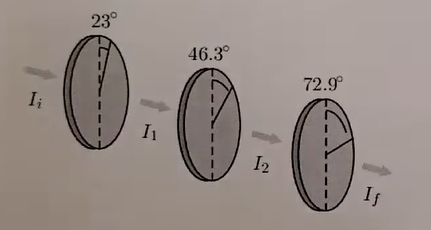
\includegraphics[width=0.5\textwidth]{13.1.PNG}
    \end{center}

    From $\phi_B = \vec{B}\cdot \vec{A}=BA\cos\theta = 10$ Wb.
\end{example}

\ex A rectangular loop of wire is moved into, through, and out of a region with a uniform magnetic field directed into the page, as shown in the figure. At Position 1, the loop has not yet entered the magnetic field. 
At Position 2, half of the loop has entered the field. At Position 3, the loop is entirely within the field. At Position 4, only half of the loop remains in the field. Compare the magnetic flux $\phi_1, \phi_2, \phi_3, \phi_4$ through the 
loop when the loop is at positions $1,2,3$, and $4$ respectively?
\begin{center}
    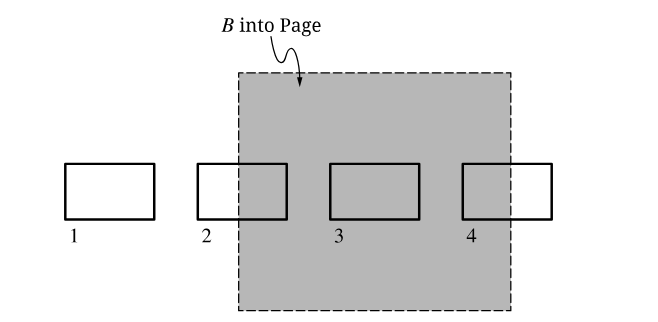
\includegraphics[width=0.5\textwidth]{13.1.1.PNG}
\end{center}

\pagebreak
\ex A four-faced pyramid whose faces are comprised of equilaterial triangles is at rest on a horizontal table. The pyramid is composed of a material that does not interact with magnetic fields. A uniform magnetic field of constant magnitude $B$ 
is directed vertically downward throughout the entire region shown. If the area of each face of the pyramid is $A$, what is the net magnetic flux passing through the top three surfaces of the pyramid that are not in contact with the table?
\begin{center}
    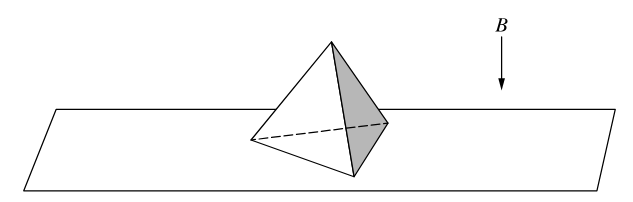
\includegraphics[width=0.5\textwidth]{13.1.2.PNG}
\end{center}

\section{Electromagnetic Induction}
Faraday's law describes the relationship between changing magnetic flux and the resulting induced emf in a system.
\[\epsilon = \frac{-\dd\phi_B}{\dd t} = \frac{-\dd(\vec{B}-\vec{A})}{\dd t} = \frac{-\dd BA\cos\theta}{\dd t}\]

Lenz's law is used to determine the direction of an induced emf resulting from a changing magnetic flux.
\begin{itemize}
    \item An induced emf generates a current that creates a magnetic field that opposes the change in magnetic flux.
\end{itemize}

Faraday's law of induction is the third of Maxwell's equations.
\[ \epsilon = \oint \vec{E}\cdot\dd \vec{l} = \frac{\dd \phi_B}{\dd t}\]

\begin{example}
    A single loop of wire is at rest in a magnetic field that is directed into the page. The loop has a radius $r$ and a resistance of $R$. The magnetic field has a magnitude $B$ that changes 
    as a function of time $t$ according to the equation $B=\alpha t+\beta t^2, \alpha$ and $\beta$ are both positive constants in units of T/s and T/s$^2$, respectively. Derive an expression for the current in the loop as a function of time.

    We know that $I=\frac{V}{R}$.

    We know that $\epsilon = \frac{\dd \phi_B}{\dd t}=\frac{\dd \vec{B}\cdot \vec{A}}{\dd t}=\frac{\dd BA}{\dd t}=\frac{A\dd B}{\dd t}$.

    From this we take the derivative and get $(\pi r^2)(\alpha + 2\beta t)$, so $I=\frac{\pi r^2(\alpha +2\beta t)}{R}$.
\end{example}

\ex The magnitude of the magnetic field in a region of space as a function of time is $B(t)=3t^2-2t+1$. The magnetic field is directed out of the page. A circular loop in the plane of the page has a radius of $R$.
Write an equation that represents the magnitude of the induced emf $\epsilon$ in the loop as a function of time.

\pagebreak
\ex \begin{center}
    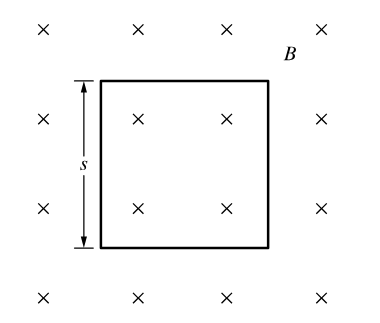
\includegraphics[width=0.5\textwidth]{13.2.PNG}
\end{center}
A single loop of wire with resistance $R$ is placed in a magnetic field that is directed into the page, as shown. The loop is a square with each side having a length $s$. The magnitude 
of the magnetic field as a function of time is given by $B(t)=4t^3+3$. What is the magnitude of the current induced in the wire due to the changing magnetic field as a function of time.

\section{Induced Currents and Magnetic Forces}
When an induced current is created in a conductive loop, the already present magnetic field will exert a magnetic force on the moving charge carriers in the loop.
\[ F_B = \int I(\dd \vec{l}\times \vec{B}) = ILB\cos\theta \]

When current is induced in a conducting loop, magnetic forces are only exerted on the segments of the loop that are within the external magnetic field.

The force on a conducting is proportional to the induced current in the loop, which depends on the rate of change of magnetic flux, the resistance 
of the loop and the velocity of the loop.

Newton's second law can be applied to a conducting loop moving in a magnetic field as it experiences an induced emf.

\begin{example}
    A rectangular loop of resistance $R$ is partly in a region of uniform magnetic field. The loop's height and length are $H$ and $l$, respectively. The magnetic field is directed out of the page.
    A constant force $F_0$ is exerted on the loop to the right such that the loop moves with constant speed $v$. Derive an expression for $v$.

    We know that $F_B=\int I(\dd l\times B)=IHB$.

    From this we solve for $I=\frac{V}{R}=\frac{1}{R}\left[\frac{\dd \phi_B}{\dd t}\right]=\frac{BHv}{R}$.

    Equating the above two gives $v=\frac{RF_0}{B^2H^2}$
\end{example}

\pagebreak
\ex \begin{center}
    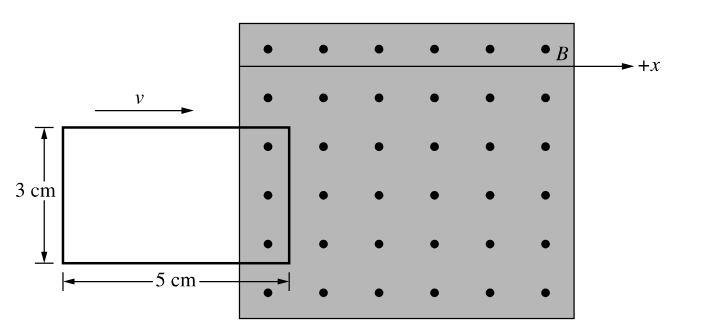
\includegraphics[width=0.5\textwidth]{13.2.1.PNG}
\end{center}
A 3.0 cm wide and 5.0 cm long rectangular loop of conducting wire of resistance $0.2\Omega$, is moved at a constant speed of 3.0 m/s to the right. The loop enters, passes through, and exits a 0.5 T 
magnetic field directed out of the page, as shown. The loop is always moved at a constant speed. What is the work done by the magnetic field on the loop?

\ex \begin{center}
    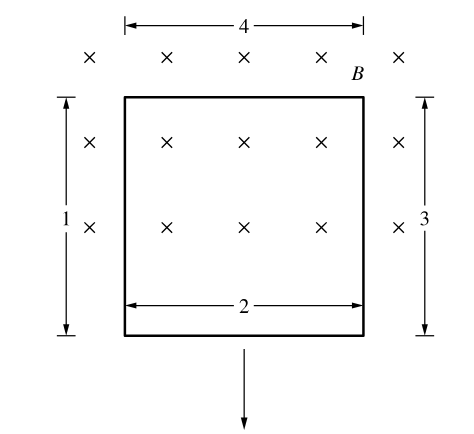
\includegraphics[width=0.5\textwidth]{13.2.2.PNG}
\end{center}
A square loop os wire is moving at speed $v$ as it exists a magnetic field directed into the page, as shown. Segments 1 and 3 of the wire are halfway in the magnetic field, Segment 2 
has completely exited the magnetic field, and Segment 4 is completely in the magnetic field. Which segment(s) of the loop, if any, will experience a magnetic force from the external magnetic field?


\section{Inductance}
Inductance is the tendency of a conductor to oppose a change in electrical current.
\begin{itemize}
    \item Depends on the physical properties of the conductor.
    \item An inductor, such as solenoid, is a circuit element that has significant inductance.
    \item The inductance of a solenoid is 
    \[ L_{sol} = \frac{\mu N^2 A}{l} \]
\end{itemize}

Inductors store energy in the magnetic field that is generated by current in the inductor.
\[ U_L = \frac{1}{2}LI^2 \]
The energy stored in the magnetic field generated by an inductor in which current is flowing can be dissipated through a resistor or used to charge a capacitor.

The transfer of energy generated in an inductor to other forms of energy obeys conservation laws.

By applying Faraday's law to an inductor and using the definition of inductance, induced emf can be related to inductance and the rate of change of current.
\[ \epsilon_i = -L \frac{\dd I}{\dd t} \]

\begin{example}
    An inductor with inductance $L=0.30$ H is connected in series with a resistor and both are connected to a power supply. The power supply generates a current that is given as a function of time $t$
    by the equation $I=I_0(1-t/k)$, where $I_0$ = 4.0 A and $k=2.0$ s. What is the magnitude of the potential difference across the inductor induced by the changing current?

    We know that $\epsilon = L\frac{\dd I}{\dd t}$. 

    To find $\frac{\dd I}{\dd t}$ we know this is equal to $\frac{\dd}{\dd t}\left[ I_0\left(1-\frac{t}{k}\right)\right]$. This is equal to $-2$.

    The answer is therefore $0.60$ V.
\end{example}

\ex What combination of physical changes to a solenoid would definitely cause an increase in its inductance?

\ex The current as a function of time in a circuit that includes an inductor of inductance $L$ is given by the equation $I=C\sqrt{t}$, where $C$ is a positive constant with appropriate units.
What is an equation for the emf $\epsilon$ across the inductor as a function of time?

\section{LR Circuits}
A resistor will dissipate energy that was stored in an inductor as the current charges.

Kirchhoff's loop rule can be applied to a series LR circuit with a bettery emf $\epsilon$, resulting in a differential equation that describes the current in the loop.
\[ \epsilon = IR + L\frac{\dd I}{\dd t}\]
The time constant is a significant feature of the behavior of an LR circuit.

The time constant of a circuit is a measure of how quickly an LR circuit will reach a steady state and is described with the equation 
\[ \tau = \frac{L}{R}\]

The electric properties of inductors change during the time interval in which the current in the inductor changes, but will 
exhibit steady state behavior after a long time interval.

\pagebreak
\begin{example}
    After a long time of the switch being closed, it is now opened. Derive an equation to show that the equation or the current as a function of time is $I=I_0e^{-t/\tau}$ where $\tau=L/R^2$.
    \begin{center}
        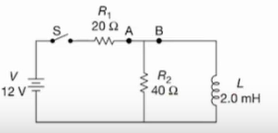
\includegraphics[width=0.5\textwidth]{13.5.PNG}
    \end{center}

    We start with $V_L-V_R = 0 \implies -L\frac{\dd I}{\dd t}-IR_2=0$.

    We can get the differential equation $\int_{I_0}^{I(t)}\frac{\dd I}{I}=\int_0^t \frac{-R_2}{L}\dd t$.
    
    Solving this equation gives $\ln I(t)-\ln I_0=-\frac{R_2}{L}t$.

    The simplification is left to the reader but it is equivalent to $I(t)=I_0e^{-t/\tau}$.
\end{example}

\ex \begin{center}
    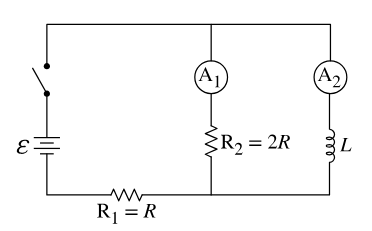
\includegraphics[width=0.5\textwidth]{13.5.1.PNG}
\end{center}
A circuit containing an inductor of inductance $L$, resistors $R_1$ and $R_2$ of resistance $R$ and $2R$, respectively, a battery of emf $\epsilon$, two ammeters, and a switch is constructed as shown in the diagram.
After the switch is closed and the circuit reaches steady state, how does the current $I_1$ measured by Ammeter $A_1$ compare to the current $I_2$ measured by Ammeter $A_2$, and why?

\pagebreak
\ex \begin{center}
    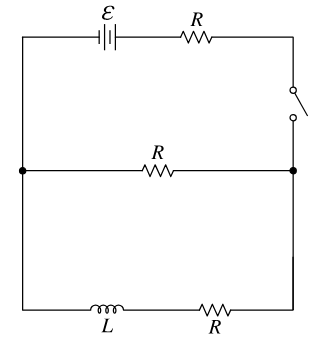
\includegraphics[width=0.5\textwidth]{13.5.2.PNG}
\end{center}
A circuit is constructed from a battery of emf $\epsilon$, a switch, an inductor of inductance $L$, and three identical resistors of resistance $R$, connected as shown in the diagram. The switch is initially open.
Write an expression that best indicates the energy stored in the inductor a long time after the switch has been closed.

\section{LC Circuits}
In circuits containing only a charged capacitor and an inductor (LC Circuits), the maximum current in the inductor 
can be determined using conservation of energy within the circuit.

In LC circuits, the time dependence of the charge stroed in the capacitor can be modeled as simple harmonic motion:
\[ \frac{\dd^2 q}{\dd t^2} = -\frac{I}{LC}q \]

The angular frequency of an oscillating LC circuit can be derived from the differnetial equation that describes an LC circuit.
\[ \omega = \frac{1}{\sqrt{LC}} \implies \omega = \frac{2\pi}{T} \implies T = \frac{2\pi}{\omega} = 2\pi\sqrt{LC}\]

\begin{example}
    A 50 $\mu$F capacitor is fully charged to 40 $\mu$C and then connected in series to a 20 mH inductor and an open switch. After the switch is closed, what is the maximum current through the inductor?

    We know that $Q=CV$ and $U_C=\frac{1}{2}CV^2$.

    From $U_C=U_L$, we get that $\frac{Q^2}{LC}=I^2$.

    Solving for $I$ and plugging in numbers gives us 0.04 A.
\end{example}

\ex A capacitor is charged using a battery until the energy stored in the electric field between the plates is equal to $U$. The capacitor is removed from the battery and then connected to an inductor.
The time it takes for the capacitor to discharge with the same initial polarity is $T$. At what time will the energy stored in the magnetic field of the inductor be equal to $U$?

\pagebreak
\ex \begin{center}
    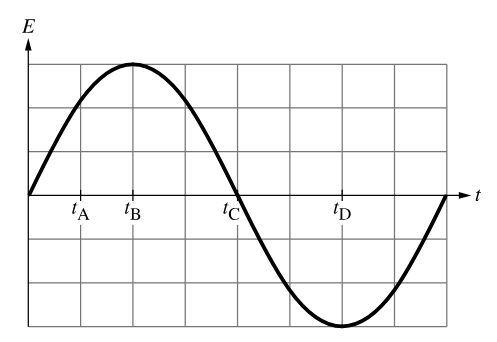
\includegraphics[width=0.5\textwidth]{13.6.PNG}
\end{center}
A circuit is constructed by connecting a capacitor and an inductor. The electric field $E$ in the capacitor varies sinusoidally with time $t$. Times $t_A, t_B, t_C$, and $t_D$ are indicated in the figure.
Rank the magnitudes of the currents $I_A, I_B, I_C$ and $I_D$ in the inductor at times $t_A, t_B, t_C$, and $t_D$ respectively.

\end{document}